\documentclass[12pt,a4paper]{article}
\usepackage[utf8]{inputenc}
\usepackage[T1]{fontenc}
\usepackage[english]{babel}
\usepackage[margin=2.5cm]{geometry}
\usepackage{enumitem}
\usepackage{booktabs}
\usepackage{hyperref}
\usepackage{xcolor}
\usepackage{parskip}
\usepackage{tikz}
\usetikzlibrary{arrows.meta, positioning, shapes.geometric}

\hypersetup{colorlinks=true, linkcolor=blue!60!black, citecolor=blue!60!black, urlcolor=blue!60!black}

\title{\textbf{Study Concept: Financial Education Before Parenthood}\\[0.3em]
\large Complexity, Dimension-Dropping, and the Case for Targeted Information\\[0.2em]
Pilot Design and Main Experiment}
\author{Draft -- April 2026}
\date{}

\begin{document}
\maketitle
\thispagestyle{empty}

% ================================================================
\section{Motivation}
% ================================================================

The transition to parenthood is one of the most consequential financial events in a woman's life. Research on the child penalty (Kleven et al., 2019) documents large and persistent earnings losses for mothers, driven primarily by reductions in working hours and occupational downgrading. Costa-Ram\'on et al.\ (2024) show that \emph{inattention} to the future contributes to suboptimal labor supply decisions after childbirth.

We build on this literature but propose a different mechanism. Our starting point is that the financial planning problem around childbirth is \textbf{inherently complex}: expectant parents must simultaneously decide on parental leave duration, Elterngeld variant (Basiselterngeld vs.\ ElterngeldPlus), tax class allocation, planned working hours after return, childcare arrangements, and the division of caregiving with their partner. These decisions \emph{interact}---the optimal Elterngeld variant depends on planned working hours, which depend on childcare availability, which depends on the partner's arrangement---creating a high-dimensional optimization problem.

\subsection{Dimension-Dropping as a Rational Response to Complexity}

We argue that the core behavioral response to this complexity is not inattention, but \textbf{strategic dimension-dropping}. When faced with an $n$-dimensional decision problem where $n$ is too large to optimize jointly, agents adopt a rational heuristic: they \emph{drop} the dimensions that are hardest to evaluate, knowing that the resulting solution will be imperfect. This is conceptually related to rational inattention (Sims, 2003) but operates at the level of problem structure rather than information acquisition: agents are aware that the dropped dimensions exist and matter, but they choose not to integrate them into their decision because the cognitive cost of doing so exceeds the perceived marginal benefit.

Which dimensions get dropped? In the parenthood context, the answer is predictable: \emph{long-term, cross-dimensional} consequences are the first to go. Estimating pension losses requires compounding effects over decades. Evaluating tax class interactions requires understanding marginal rates, benefit phase-outs, and their interaction with the partner's income. Projecting career trajectory costs requires modeling counterfactual scenarios. By contrast, applying for Elterngeld, planning the first-year budget, and arranging maternity leave are \emph{proximate, single-dimensional} problems that can be solved in isolation. The complexity of the decision environment therefore systematically channels attention toward the short run.

Crucially, this is not ignorance. Mothers may well be \emph{vaguely aware} that part-time work reduces their pension, or that tax class choices have long-run implications. The problem is that converting this vague awareness into actionable planning requires solving the very cross-dimensional optimization that complexity makes intractable. The knowledge gap arises not from missing information per se, but from the inability to \emph{integrate} information across dimensions.

\subsection{The U-Shape: Complexity and Engagement}

This mechanism predicts a non-monotonic relationship between topic complexity and engagement. At low complexity, people discuss, plan, and decide freely. As complexity increases, initial engagement rises---people recognize the importance and try harder. But past a threshold, engagement \emph{collapses}: the topic feels too difficult to reason about productively, and people stop talking about it, stop planning around it, and default to whatever simple, socially available script exists.

In the German context, the socially available script is the traditional norm: take extended parental leave, return part-time, let the higher-earning partner (typically the father) maximize household income in the short run. The critical insight is that \textbf{complexity reduction and norm-following align}: when dropping complex long-term dimensions from the decision, the remaining simple dimensions often point toward the norm. What looks like a traditional \emph{preference} may, in many cases, be the residual of a complexity-induced optimization failure. The U-shape implies that the most consequential financial dimensions---precisely those where information could help most---are the ones people engage with least.

\subsection{Implications for Intervention Design}

This framework yields a clear prediction: information that merely \emph{reminds} women to think about the future (a salience intervention) should have limited effect, because the problem is not that they have forgotten but that they cannot compute. Effective intervention must \emph{reduce complexity}---translate high-dimensional trade-offs into concrete, single-dimensional comparisons that can be integrated into an already complex decision. For example, turning ``part-time work is bad for your pension'' into ``10 years of half-time costs you approximately 150--200\,\texteuro/month in retirement'' collapses a multi-decade, multi-variable calculation into one number.

Through a cooperation with Keleya, a pregnancy app used widely in Germany, we can reach expectant mothers during pregnancy---the precise window in which plans about parental leave, return-to-work timing, and working hours are formed, and where dimension-dropping has not yet hardened into revealed behavior.

% ================================================================
\section{Conceptual Framework}
% ================================================================

The following diagram illustrates the dimension-dropping mechanism and how the treatment intervenes:

\begin{center}
\resizebox{\textwidth}{!}{%
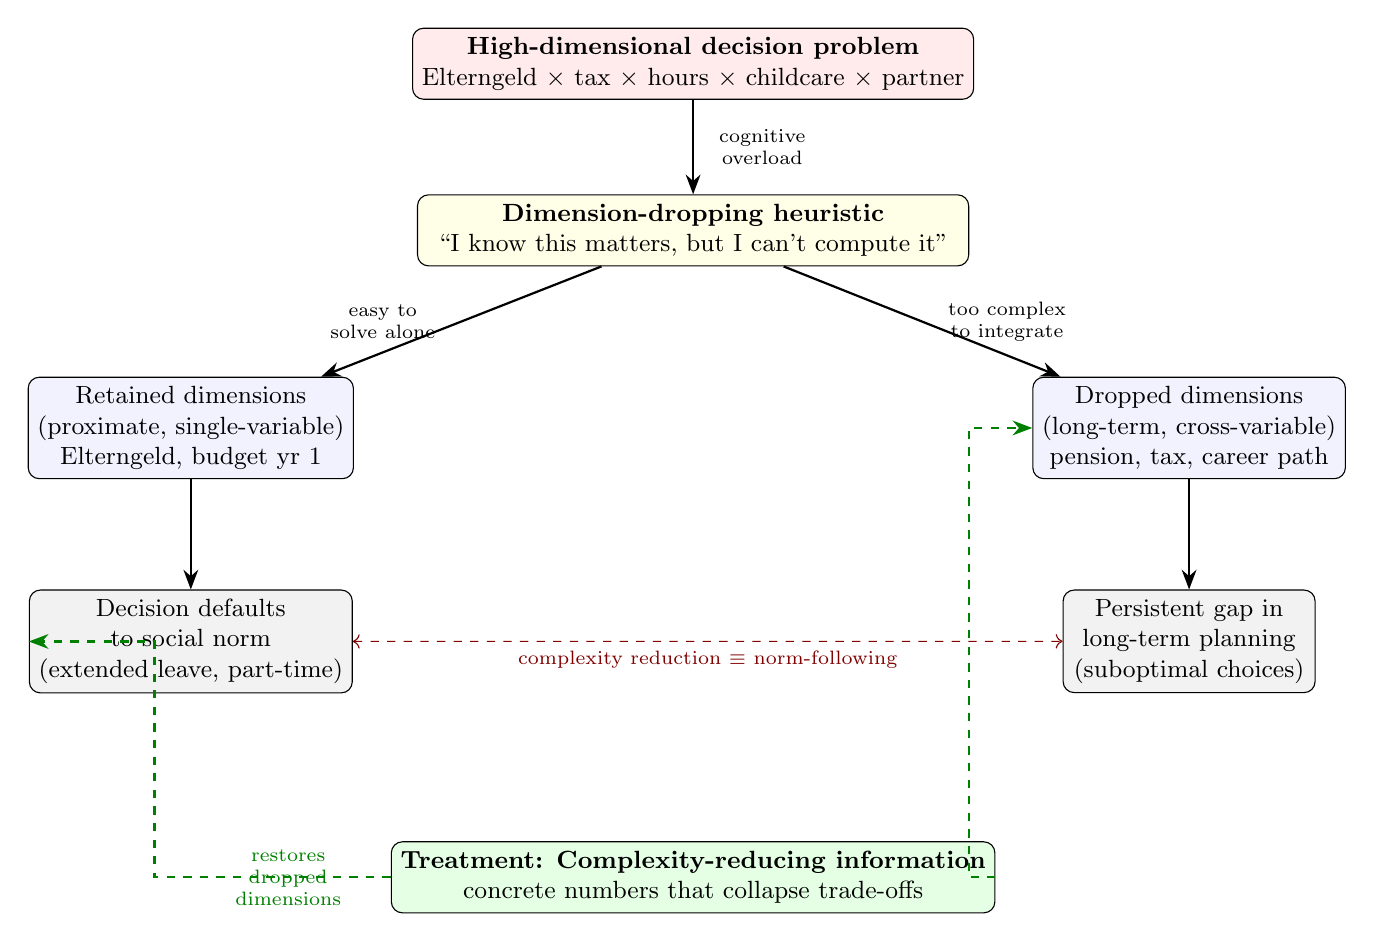
\begin{tikzpicture}[
    node distance=1.2cm and 2.5cm,
    every node/.style={align=center, font=\small},
    box/.style={draw, rounded corners, minimum width=3.2cm, minimum height=0.9cm, fill=blue!5},
    wide/.style={draw, rounded corners, minimum width=7cm, minimum height=0.9cm, fill=orange!8},
    arrow/.style={-{Stealth[length=2.5mm]}, thick}
]

% Top: complexity
\node[wide, fill=red!8] (complex) {\textbf{High-dimensional decision problem}\\Elterngeld $\times$ tax $\times$ hours $\times$ childcare $\times$ partner};

% Rational response
\node[wide, below=1.2cm of complex, fill=yellow!10] (drop) {\textbf{Dimension-dropping heuristic}\\``I know this matters, but I can't compute it''};

\draw[arrow] (complex) -- node[right, font=\scriptsize, xshift=2mm] {cognitive\\overload} (drop);

% Two resulting states
\node[box, below left=1.4cm and 0.8cm of drop] (short) {Retained dimensions\\(proximate, single-variable)\\Elterngeld, budget yr 1};
\node[box, below right=1.4cm and 0.8cm of drop] (dropped) {Dropped dimensions\\(long-term, cross-variable)\\pension, tax, career path};

\draw[arrow] (drop) -- node[left, font=\scriptsize, xshift=-2mm] {easy to\\solve alone} (short);
\draw[arrow] (drop) -- node[right, font=\scriptsize, xshift=2mm] {too complex\\to integrate} (dropped);

% Norm alignment
\node[box, below=1.4cm of short, fill=gray!10] (norm) {Decision defaults\\to social norm\\(extended leave, part-time)};
\node[box, below=1.4cm of dropped, fill=gray!10] (gap) {Persistent gap in\\long-term planning\\(suboptimal choices)};

\draw[arrow] (short) -- (norm);
\draw[arrow] (dropped) -- (gap);

% U-shape annotation
\draw[<->, dashed, color=red!50!black] (norm) -- node[below, font=\scriptsize] {complexity reduction $\equiv$ norm-following} (gap);

% Intervention
\node[wide, below=1.8cm of drop, yshift=-5.5cm, fill=green!10] (treat) {\textbf{Treatment: Complexity-reducing information}\\concrete numbers that collapse trade-offs};

\draw[arrow, dashed, color=green!50!black] (treat) -- ++(3.5,0) |- (dropped);
\draw[arrow, dashed, color=green!50!black] (treat.west) -- ++(-0.5,0) node[left, font=\scriptsize, color=green!50!black] {restores\\dropped\\dimensions} -- ++(-2.5,0) |- (norm);

\end{tikzpicture}%
}% end resizebox
\end{center}

The treatment works by converting dropped dimensions into tractable ones: it does not merely add information but \emph{changes the dimensionality} of the retained decision problem. By presenting long-term consequences as concrete, single-number comparisons, it makes these dimensions as easy to integrate as the short-term ones---effectively un-dropping them. If this succeeds, the decision should shift away from the norm-default and toward a more personally optimized outcome.

% ================================================================
\section{Research Question}
% ================================================================

Can targeted, complexity-reducing financial information about the \emph{long-term} consequences of parenthood---delivered before childbirth---shift beliefs, plans, and ultimately labor market behavior of mothers? And does the effect operate through dimension restoration (making dropped trade-offs tractable) rather than mere salience (reminding women to think about the future)?

% ================================================================
\section{Study Design}
% ================================================================

\subsection{Sample and Access}

Through Keleya, we have access to approximately:
\begin{itemize}[nosep]
    \item \textbf{800 pregnant women} (pre-birth)---the main experimental sample
    \item \textbf{1{,}600 recent mothers} (post-birth)---for baseline calibration and potential second experiment
\end{itemize}

\subsection{Experimental Arms (Pre-Birth Sample)}

Pregnant women are randomly assigned to one of three conditions:

\begin{table}[h]
\centering
\begin{tabular}{@{}lp{10cm}@{}}
\toprule
\textbf{Arm} & \textbf{Content} \\
\midrule
Control & Baseline survey only (no information provided) \\[0.5em]
Short-term Info & Information that expectant parents typically seek---the dimensions they already \emph{retain}: parental leave benefit calculation (Elterngeld), maternity protection periods, first-year household budget planning \\[0.5em]
Long-term Info & Information on the dimensions typically \emph{dropped}: child penalty in concrete numbers, pension effect of 10 years part-time work, tax class interaction effects on work incentives (Ehegattensplitting), long-run career costs of reduced hours---presented as \emph{concrete, single-number scenarios} designed to make these dimensions as tractable as short-term ones \\
\bottomrule
\end{tabular}
\end{table}

The comparison between Long-term and Short-term Info is the key identification: both arms receive financial education of comparable length and quality, but with different \emph{time horizons}. This isolates the effect of information content from the effect of receiving any information at all.

The dimension-dropping framework sharpens the interpretation: the Short-term arm reinforces dimensions women already retain in their decision. The Long-term arm \emph{restores} dimensions that complexity caused them to drop. The prediction is that only the Long-term arm should shift behavior, because the Short-term information is redundant with the dimensions already being optimized.

\subsection{Primary Outcomes (Measured Immediately Post-Treatment)}

\begin{enumerate}[nosep]
    \item \textbf{Beliefs:} Estimated pension loss from 10 years of part-time work; estimated income loss over a decade; perceived financial consequences of different working-hour scenarios
    \item \textbf{Plans:} Planned timing of return to work; planned weekly hours; planned parental leave split with partner
    \item \textbf{Knowledge:} Factual questions on pension mechanics, tax splitting effects
    \item \textbf{Perceived complexity:} Self-reported difficulty of financial planning around childbirth. If the Long-term arm reduces perceived complexity more than the Short-term arm, the dimension-restoration mechanism is directly supported: the treatment worked not by adding more to think about, but by making what was there more tractable
    \item \textbf{Engagement shift:} Willingness to discuss or seek information on long-term financial topics (tests the U-shape prediction---if complexity is reduced, engagement with previously avoided topics should increase)
\end{enumerate}

\subsection{Secondary Outcomes (Follow-up at 6--12 Months Post-Birth)}

\begin{enumerate}[nosep]
    \item Actual return-to-work timing and working hours
    \item Actual parental leave split with partner
    \item Retrospective satisfaction with the decision
    \item Whether participants sought additional financial information or advice between treatment and follow-up
\end{enumerate}

Follow-up is feasible through Keleya's continued engagement with users after birth.

\subsection{Role of Recent Mothers (n\,=\,1{,}600)}

Two possible uses:
\begin{enumerate}[nosep]
    \item \textbf{Descriptive baseline:} Revealed-preference data on what actually surprised mothers, which factors mattered most, how large the expectation--reality gap is. This calibrates the treatment content and provides direct evidence for dimension-dropping: if the topics that \emph{surprised} mothers most (B2) are systematically absent from what they \emph{worried about} before birth (A0b), the dropped dimensions are empirically identified.
    \item \textbf{Second experiment:} Randomized treatment among mothers still in parental leave who face the return-to-work decision. This provides a second decision margin (closer to the actual choice) and a separate paper or robustness check.
\end{enumerate}

% ================================================================
\section{Contribution and Positioning}
% ================================================================

\begin{table}[h]
\centering
\small
\begin{tabular}{@{}p{3.8cm}p{4.2cm}p{5.5cm}@{}}
\toprule
& \textbf{Costa-Ram\'on et al.} & \textbf{This paper} \\
\midrule
Mechanism & Inattention to future & Complexity-induced dimension-dropping \\[0.3em]
Nature of the problem & Women don't think about the future & Women \emph{know} it matters but cannot integrate the long-term dimensions into a tractable decision \\[0.3em]
Intervention logic & Salience: prompt women to think about the future & Complexity reduction: make dropped dimensions tractable by collapsing them into concrete numbers \\[0.3em]
Timing & Post-birth (retrospective) & Pre-birth (prospective, before decisions are locked in) \\[0.3em]
Key comparison & Attention vs.\ no attention & Long-term info vs.\ short-term info (both are ``education'') \\[0.3em]
Norm interaction & Not addressed & Dimension-dropping defaults to social norm; treatment breaks this alignment \\[0.3em]
Policy implication & Nudge mothers to think ahead & Provide specific, complexity-reducing knowledge at the right time \\
\bottomrule
\end{tabular}
\end{table}

\noindent The complexity framing connects to a broader literature on decision-making under complexity (Handel and Kolstad, 2015; Bhargava and Manoli, 2015), rational inattention (Sims, 2003; Matejka and McKay, 2015), and financial literacy (Lusardi and Mitchell, 2014; Laudenbach et al.). The theoretical contribution is to show how complexity operates not through general ``confusion'' but through a structured process of dimension-dropping that systematically disadvantages the long-term. The empirical contribution is to show that \emph{targeted} financial education---designed to restore the specific dropped dimensions---can shift real economic decisions at scale.

% ================================================================
\section{Role of the Pilot Study}
% ================================================================

The pilot survey (conducted with experienced mothers via oTree) serves five functions:

\subsection{Identifying Which Dimensions Get Dropped}

The pilot now includes a structured two-stage elicitation. First, open-text questions (A0.4, A0.5) capture what mothers thought about before birth and what they wish they had thought about---without priming. Then, a structured worry ranking (A0b) asks mothers to rank their pre-birth concerns across predefined categories spanning short-term (health, birth) to long-term (pension, career, financial security).

The key analytical comparison is between A0b and B2. A0b measures which dimensions mothers \emph{retained} before birth; B2 measures which financial topics \emph{surprised} them after. If A0b worries cluster on short-term, proximate topics while B2 surprises cluster on long-term, cross-dimensional ones, the dimension-dropping mechanism is directly identified in the pilot data.

\subsection{Testing the U-Shape}

The open-text questions (A0.4, A0.5, A1) provide qualitative evidence on the U-shape prediction. If respondents write extensively about simple topics (health, the birth itself) but give only brief or vague answers about financial planning, this is consistent with engagement collapsing above a complexity threshold. The structured A0b ranking can test this quantitatively: long-term financial categories should appear less frequently despite being consequential.

\subsection{Calibrating Treatment Content}

Questions A2 and B2 ask mothers to rank the factors that most affected their return to work and the financial topics that most surprised them. The ranking data directly determines which long-term topics to include in the treatment:

\begin{itemize}[nosep]
    \item If pension effects rank highly as surprising $\rightarrow$ include pension scenario in Long-term Info
    \item If tax/benefit interactions rank highly $\rightarrow$ include Ehegattensplitting explainer
    \item If childcare costs dominate $\rightarrow$ this is a retained (short-term) dimension and belongs in the Short-term arm
\end{itemize}

The new B1b question (``Did you manage financially better or worse than expected?'') and the neutral B2 reframing (``most unexpected---positive or negative'') ensure that the data captures both directions of surprise, avoiding the suggestive negative framing that could bias toward a pessimistic picture.

\subsection{Validating the Knowledge Gap}

Section D tests factual knowledge: D1 asks mothers to estimate the monthly pension loss from 10 years of part-time work (in a concrete scenario); D2 tests understanding of Ehegattensplitting---now with an embedded explanation and a ``I don't know what Ehegattensplitting is'' option, which itself reveals whether the concept is accessible. If pilot respondents---who have \emph{already experienced} parenthood---still answer incorrectly or report not knowing the concept, the dimension was not just dropped but never successfully restored through experience alone.

\subsection{Measuring the Short-Term Bias}

Question B4 (planning horizon before birth) directly tests the dimension-dropping hypothesis. If the majority of mothers report having planned primarily for the short term (pregnancy, first year), and B4b shows retrospective regret about not planning further ahead, the selective retention of proximate dimensions is empirically grounded.

The restructured Section A provides additional evidence. A4 (expected vs.\ actual return timing) now opens the section, followed by a Likert scale on overall return-to-work experience, free-text elaboration, and then a separate ranking page. This flow captures the expectation--reality gap before respondents are primed by the structured ranking categories.

The new A2 item ``Erwartungen aus meinem Umfeld'' captures whether social norms played a role---if this item ranks highly alongside long-term financial dimensions being dropped, it supports the hypothesis that complexity reduction and norm-following align.

% ================================================================
\section{What Is Needed for a Top-5 Paper}
% ================================================================

\begin{enumerate}
    \item \textbf{Clean identification:} RCT with randomization within Keleya's user base. The three-arm design (Control / Short-term / Long-term) allows for clean causal identification and rules out the alternative that \emph{any} information moves the needle.

    \item \textbf{A novel mechanism:} The dimension-dropping framework goes beyond ``inattention'' and ``financial illiteracy'' as separate explanations. It provides a unified, structured account: complexity \emph{generates} the knowledge gap (through dropping), \emph{produces} the short-term focus (through selective retention), and \emph{aligns} with social norms (making it look like preference). The three-arm design can distinguish this from pure salience effects.

    \item \textbf{Behavioral outcomes:} The follow-up data on actual working hours and parental leave split moves the paper beyond stated preferences to revealed behavior.

    \item \textbf{Policy relevance:} Pre-birth financial education as a scalable, low-cost policy tool. Germany's institutional infrastructure (universal Elterngeld, high Keleya penetration) makes this immediately implementable. The finding would generalize to any setting where a complex decision environment produces systematic dimension-dropping.

    \item \textbf{Heterogeneity analysis:} Does the treatment work differently for low- vs.\ high-income women? First-time vs.\ experienced mothers? Women in complex vs.\ simple tax situations (Steuerklasse III/V vs.\ IV/IV)? This determines \emph{who benefits most} and sharpens the mechanism: if the effect is strongest for women in objectively more complex situations (e.g., large income differences with partner, more interacting tax dimensions), the dimension-dropping mechanism is directly supported.

    \item \textbf{Mechanism evidence:} The pilot provides unusually detailed mechanism evidence across multiple layers:
    \begin{itemize}[nosep]
        \item \emph{Dimension identification:} A0b (pre-birth worries) vs.\ B2 (post-birth surprises) reveals exactly which dimensions were dropped
        \item \emph{U-shape evidence:} Open-text engagement patterns and A0b ranking frequencies test the non-monotonic complexity--engagement relationship
        \item \emph{Knowledge gap:} D1/D2 confirm that dropped dimensions remain poorly understood even after experience
        \item \emph{Norm alignment:} A2 (social expectations item) and the overall pattern of retained vs.\ dropped dimensions test whether default decisions follow social norms
        \item \emph{Complexity reduction (main experiment):} Perceived complexity as an outcome variable directly tests whether the treatment works by reducing dimensionality
    \end{itemize}
\end{enumerate}

% ================================================================
\section{Timeline}
% ================================================================

\begin{table}[h]
\centering
\begin{tabular}{@{}ll@{}}
\toprule
\textbf{Phase} & \textbf{Timing} \\
\midrule
Pilot survey (experienced mothers) & Spring 2026 \\
Treatment content development (based on pilot) & Summer 2026 \\
Pre-registration (AEA RCT Registry) & Late summer 2026 \\
Main experiment via Keleya (pre-birth sample) & Autumn 2026 \\
Follow-up survey (6--12 months post-birth) & Spring--Autumn 2027 \\
Analysis and paper draft & Late 2027 \\
\bottomrule
\end{tabular}
\end{table}

\end{document}
